\documentclass[ignorenonframetext]{beamer}
\usetheme{sts}
\title[HW-7-2]{Homework Sheet 7, Ex. 2}

\author{Büchler P., Lohmann N.J}
\institute{Institute for Software Systems}
\date{\today}

\begin{document}

\begin{document}
\newcommand{\slide1}{%
\begin{frame}<presentation>[plain]
\titlepage{}
\end{frame}
}


\newcommand{\slide2}{
\begin{frame}<presentation>
\frametitle{Contents}
%\tableofcontents[hideallsubsections]{}
\tableofcontents[]{}
\end{frame}
}

\section{Ex.2}
\subsection{Data Flow}


\begin{frame}{Data Flow Graph}
\begin{figure}[h]    
\centering
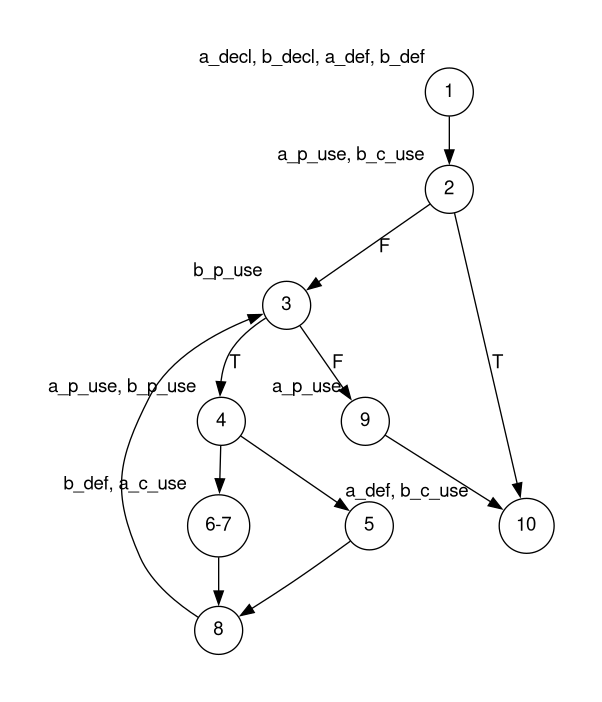
\includegraphics[scale=0.3]{dataflowgraph.png}
\end{figure}
\end{frame}

\begin{frame}


\frametitle{DU-Paths (a)}
\begin{itemize}
\item 1-2, 1-2-3-9
\item 1-2-3-4, 1-2-3-4-6-7, 1-2-3-4-6-7-9
\item 5-8-3-4,  5-8-3-4-6-7 
\item 5-8-3-9
\end{itemize}
\end{frame}

\begin{frame}
\frametitle{DU-Paths (b)}
\begin{itemize}
\item 1-2, 1-2-3
\item 1-2-3-4, 1-2-3-4-5
\item 6-7-8-3, 6-7-8-3-4, 6-7-8-3-4-5 
\end{itemize}
\end{frame}

\subsection{Test Suite}

\begin{frame}{Test Suite}
\begin{tabular}{c c}
Test      & \#1          \\
Test Path & 1-2          \\
Coverage  & 1-2          \\
Input     & a = 0, b = 0 \\
Output    & 0             
\end{tabular}

\noindent\makebox[\linewidth]{\rule{\paperwidth}{0.4pt}}

\begin{tabular}{c c}
Test      & \#2          \\
Test Path & 1-2-3-9          \\
Coverage  & 1-2, 1-2-3-9          \\
Input     & a = 1, b = 0 \\
Output    & 1             
\end{tabular}
\end{frame}

\begin{frame}{Test Suite cont.}
\begin{tabular}{c c}
Test      & \#3          \\
Test Path & 1-2-3-4-6-7-8-3-9          \\
Coverage  & 1-2, 1-2-3-4, 1-2-3-4-6-7, 1-2-3-4-6-7-8-9          \\
Input     & a = 1, b = 1 \\
Output    & 1             
\end{tabular}

\noindent\makebox[\linewidth]{\rule{\paperwidth}{0.4pt}}

\begin{tabular}{c c}
Test      & \#4          \\
Test Path & 1-2-3-4-5-8-3-4-6-7-8-3-9          \\
Coverage  & 1-2, 1-2-3-4, 5-8-3-4, 5-8-3-4-6-7, 5-8-3-4-9         \\
Input     & a = 2, b = 1 \\
Output    & 1             
\end{tabular}
\end{frame}


\subsection{Comparison}
\begin{frame}{Comparison Data Flow vs. Branch coverage}
    For 100\% multiple-condition coverage, \(c = 3 \implies 2^c = 8\)
    \newline
    Twice the No. of Data-Flow cases, due to test cases of the form \(a = 0, b = * \).
    Which never go further than the path 1-2-3-9.
\end{frame}

\subsection{Practice}
\begin{frame}{Practice}
\center
But how does this actually look like? After all our Data Flow graphs are fortunately made for us humans and hence subjective!, but a compiler needs to be precise.
DU-paths (commonly known as Def-Use chains) are too complex to generate but go in the right direction.
The next step are Static Single-Assignment form (SSA) derived from the CFG.
\end{frame}

\begin{frame}[fragile]
    One can generate quiet helpful information that the compiler \(gcc \geq 4.0\) uses via
    \begin{verbatim}
        gcc gcd_data_flow.c -fdump-tree-all-graph
    \end{verbatim}
    Most importantly 
    \begin{verbatim}
        gcd_data_flow.c.cfg
    \end{verbatim}
    \begin{verbatim}
        gcd_data_flow.c.ssa
    \end{verbatim}
\end{frame}

\begin{frame}
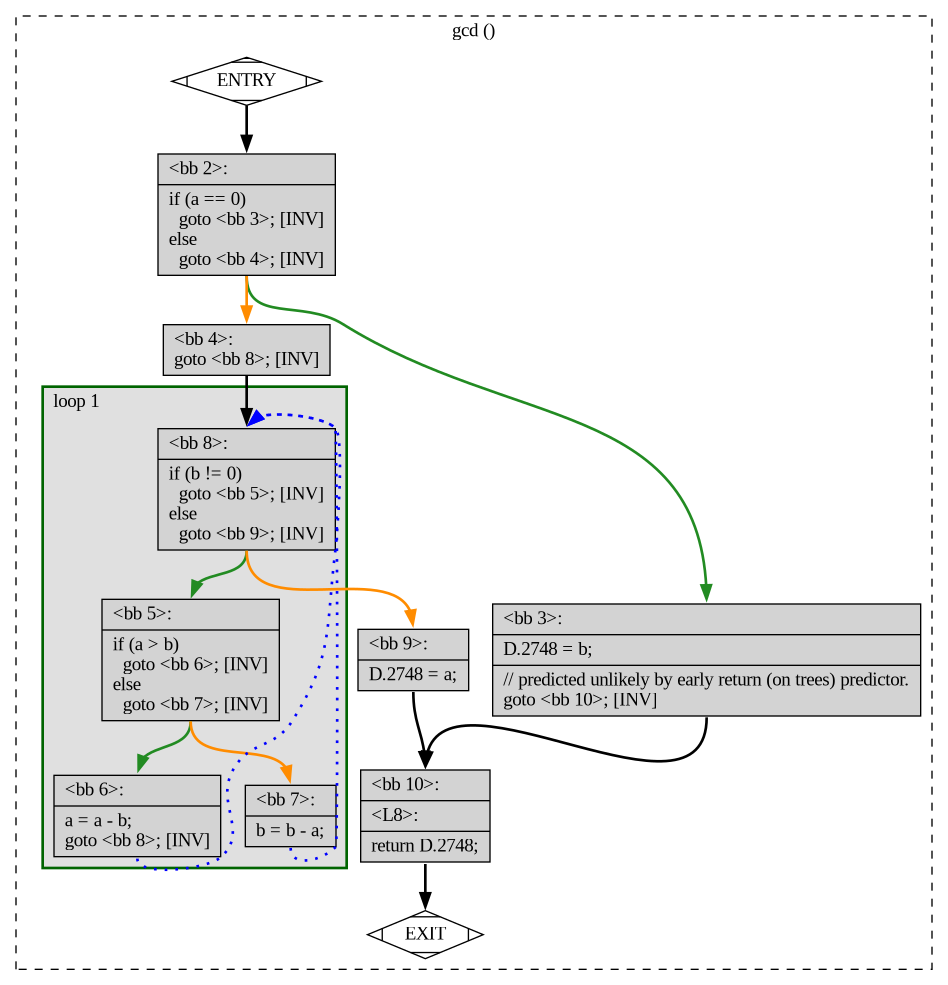
\includegraphics[scale=0.22]{gcd_data_flow_graph_cfg.png}
\end{frame}


\begin{frame}
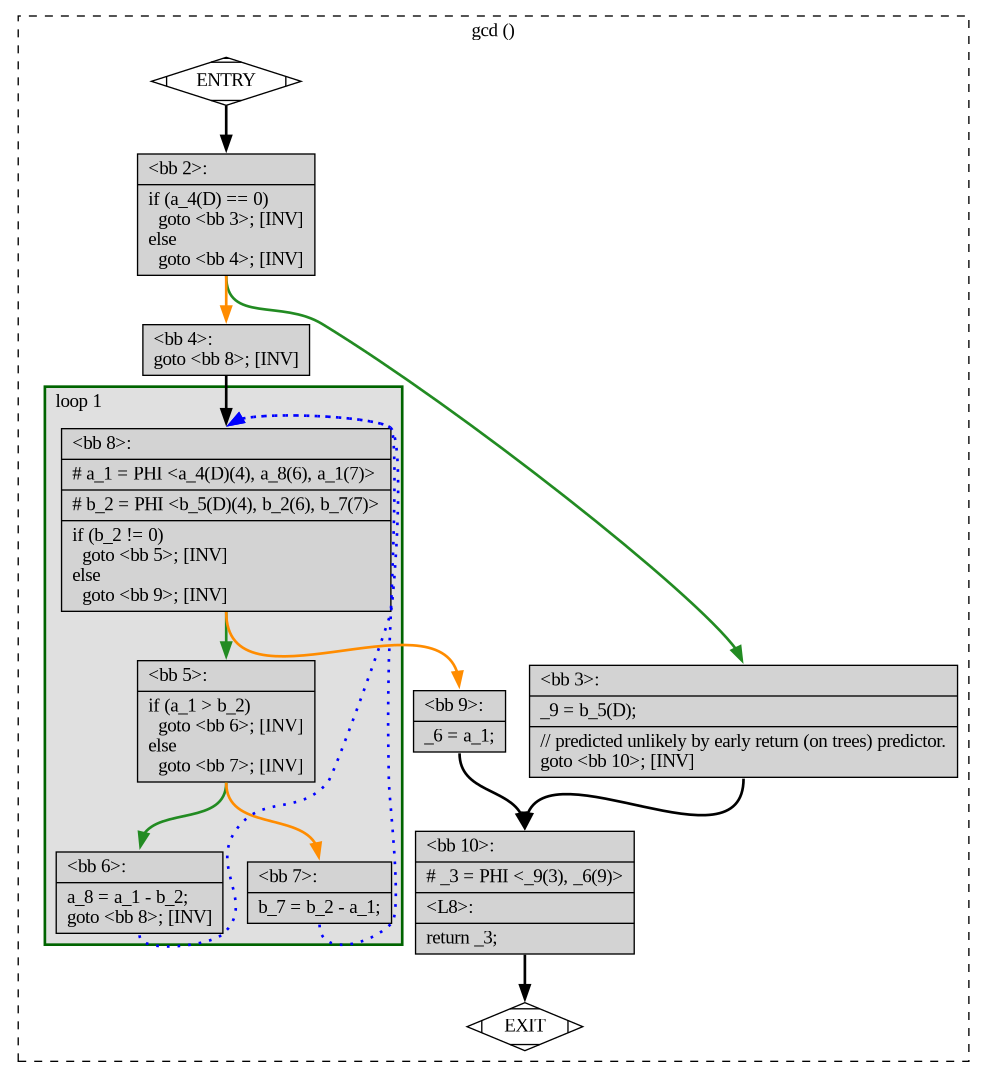
\includegraphics[scale=0.2]{gcd_data_flow_graph_ssa.png}
\end{frame}

\begin{frame}[fragile]{Coverage}
\begin{tiny}
How about the statement/decision coverage? Really dependent on the languages ecosystem and most are happy with statement coverage.
For c there is gcov available. Running
\begin{verbatim}
#include <assert.h>
unsigned gcd(unsigned a, unsigned b) {
    if (a == 0) return b;
    while (b != 0) {
        if (a > b) {
            a -= b;
        } else {
            b -= a;
    } }
    return a;
}

int main() {
    assert(gcd(0, 0) == 0);
    assert(gcd(1, 0) == 1);
    assert(gcd(1, 1) == 1);
    assert(gcd(2, 1) == 1);
    return 0;
}
\end{verbatim}
\end{tiny}
\begin{verbatim}
$ gcc -Wall -fprofile-arcs -ftest-coverage gcd_data_flow_test.c
$ ./a.out
$ gcov -b -c gcd_data_flow_test.c
\end{verbatim}
\end{frame}

\begin{frame}[fragile]
\begin{tiny}
\begin{verbatim}
    File 'gcd_data_flow_test.c'
    Lines executed:100.00% of 13
    Branches executed:100.00% of 14
    Taken at least once:71.43% of 14
    Calls executed:50.00% of 8
    Creating 'gcd_data_flow_test.c.gcov'
\end{verbatim}

\begin{verbatim}
    function gcd called 4 returned 100% blocks executed 100%
        4:    3:unsigned gcd(unsigned a, unsigned b) {
        4:    4:    if (a == 0) return b;
branch  0 taken 25% (fallthrough)
branch  1 taken 75%
        6:    5:    while (b != 0) {
branch  0 taken 50%
branch  1 taken 50% (fallthrough)
        3:    6:        if (a > b) {
branch  0 taken 33% (fallthrough)
branch  1 taken 67%
        1:    7:            a -= b;
        -:    8:        } else {
        2:    9:            b -= a;
        -:   10:    } }
        3:   11:    return a;
        -:   12:}
        -:   13:

\end{verbatim}
\end{tiny}
\end{frame}

\begin{frame}[fragile]
    \begin{tiny}
        Removing the last test gives instead
        \begin{verbatim}
    File 'gcd_data_flow_test.c'
    Lines executed:91.67% of 12
    Branches executed:100.00% of 12
    Taken at least once:66.67% of 12
    Calls executed:50.00% of 6
    Creating 'gcd_data_flow_test.c.gcov'
        \end{verbatim}
\begin{verbatim}
        function gcd called 3 returned 100% blocks executed 90%
        3:    3:unsigned gcd(unsigned a, unsigned b) {
        3:    4:    if (a == 0) return b;
branch  0 taken 33% (fallthrough)
branch  1 taken 67%
        3:    5:    while (b != 0) {
branch  0 taken 33%
branch  1 taken 67% (fallthrough)
        1:    6:        if (a > b) {
branch  0 taken 0% (fallthrough)
branch  1 taken 100%
    #####:    7:            a -= b;
        -:    8:        } else {
        1:    9:            b -= a;
        -:   10:    } }
        2:   11:    return a;
        -:   12:}
        \end{verbatim}
    \end{tiny}
\end{frame}

\subsection{Thanks}
\begin{frame}{The End}
    \center 
    Thank you for your attention!
\end{frame}

\end{document}
